\mySection{11.1 Introduction}
%-------------- start slide -------------------------------%{{{ 11.4
\begin{frame}
	% {\S\: 11.1 Introduction}
	\begin{center}
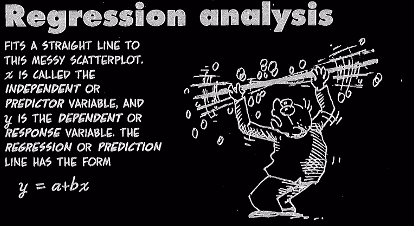
\includegraphics[scale=2]{cartoon_guide_regression-neg.png}
\vspace{2em}
\footnotesize
\url{https://madhureshkumar.wordpress.com/}
% 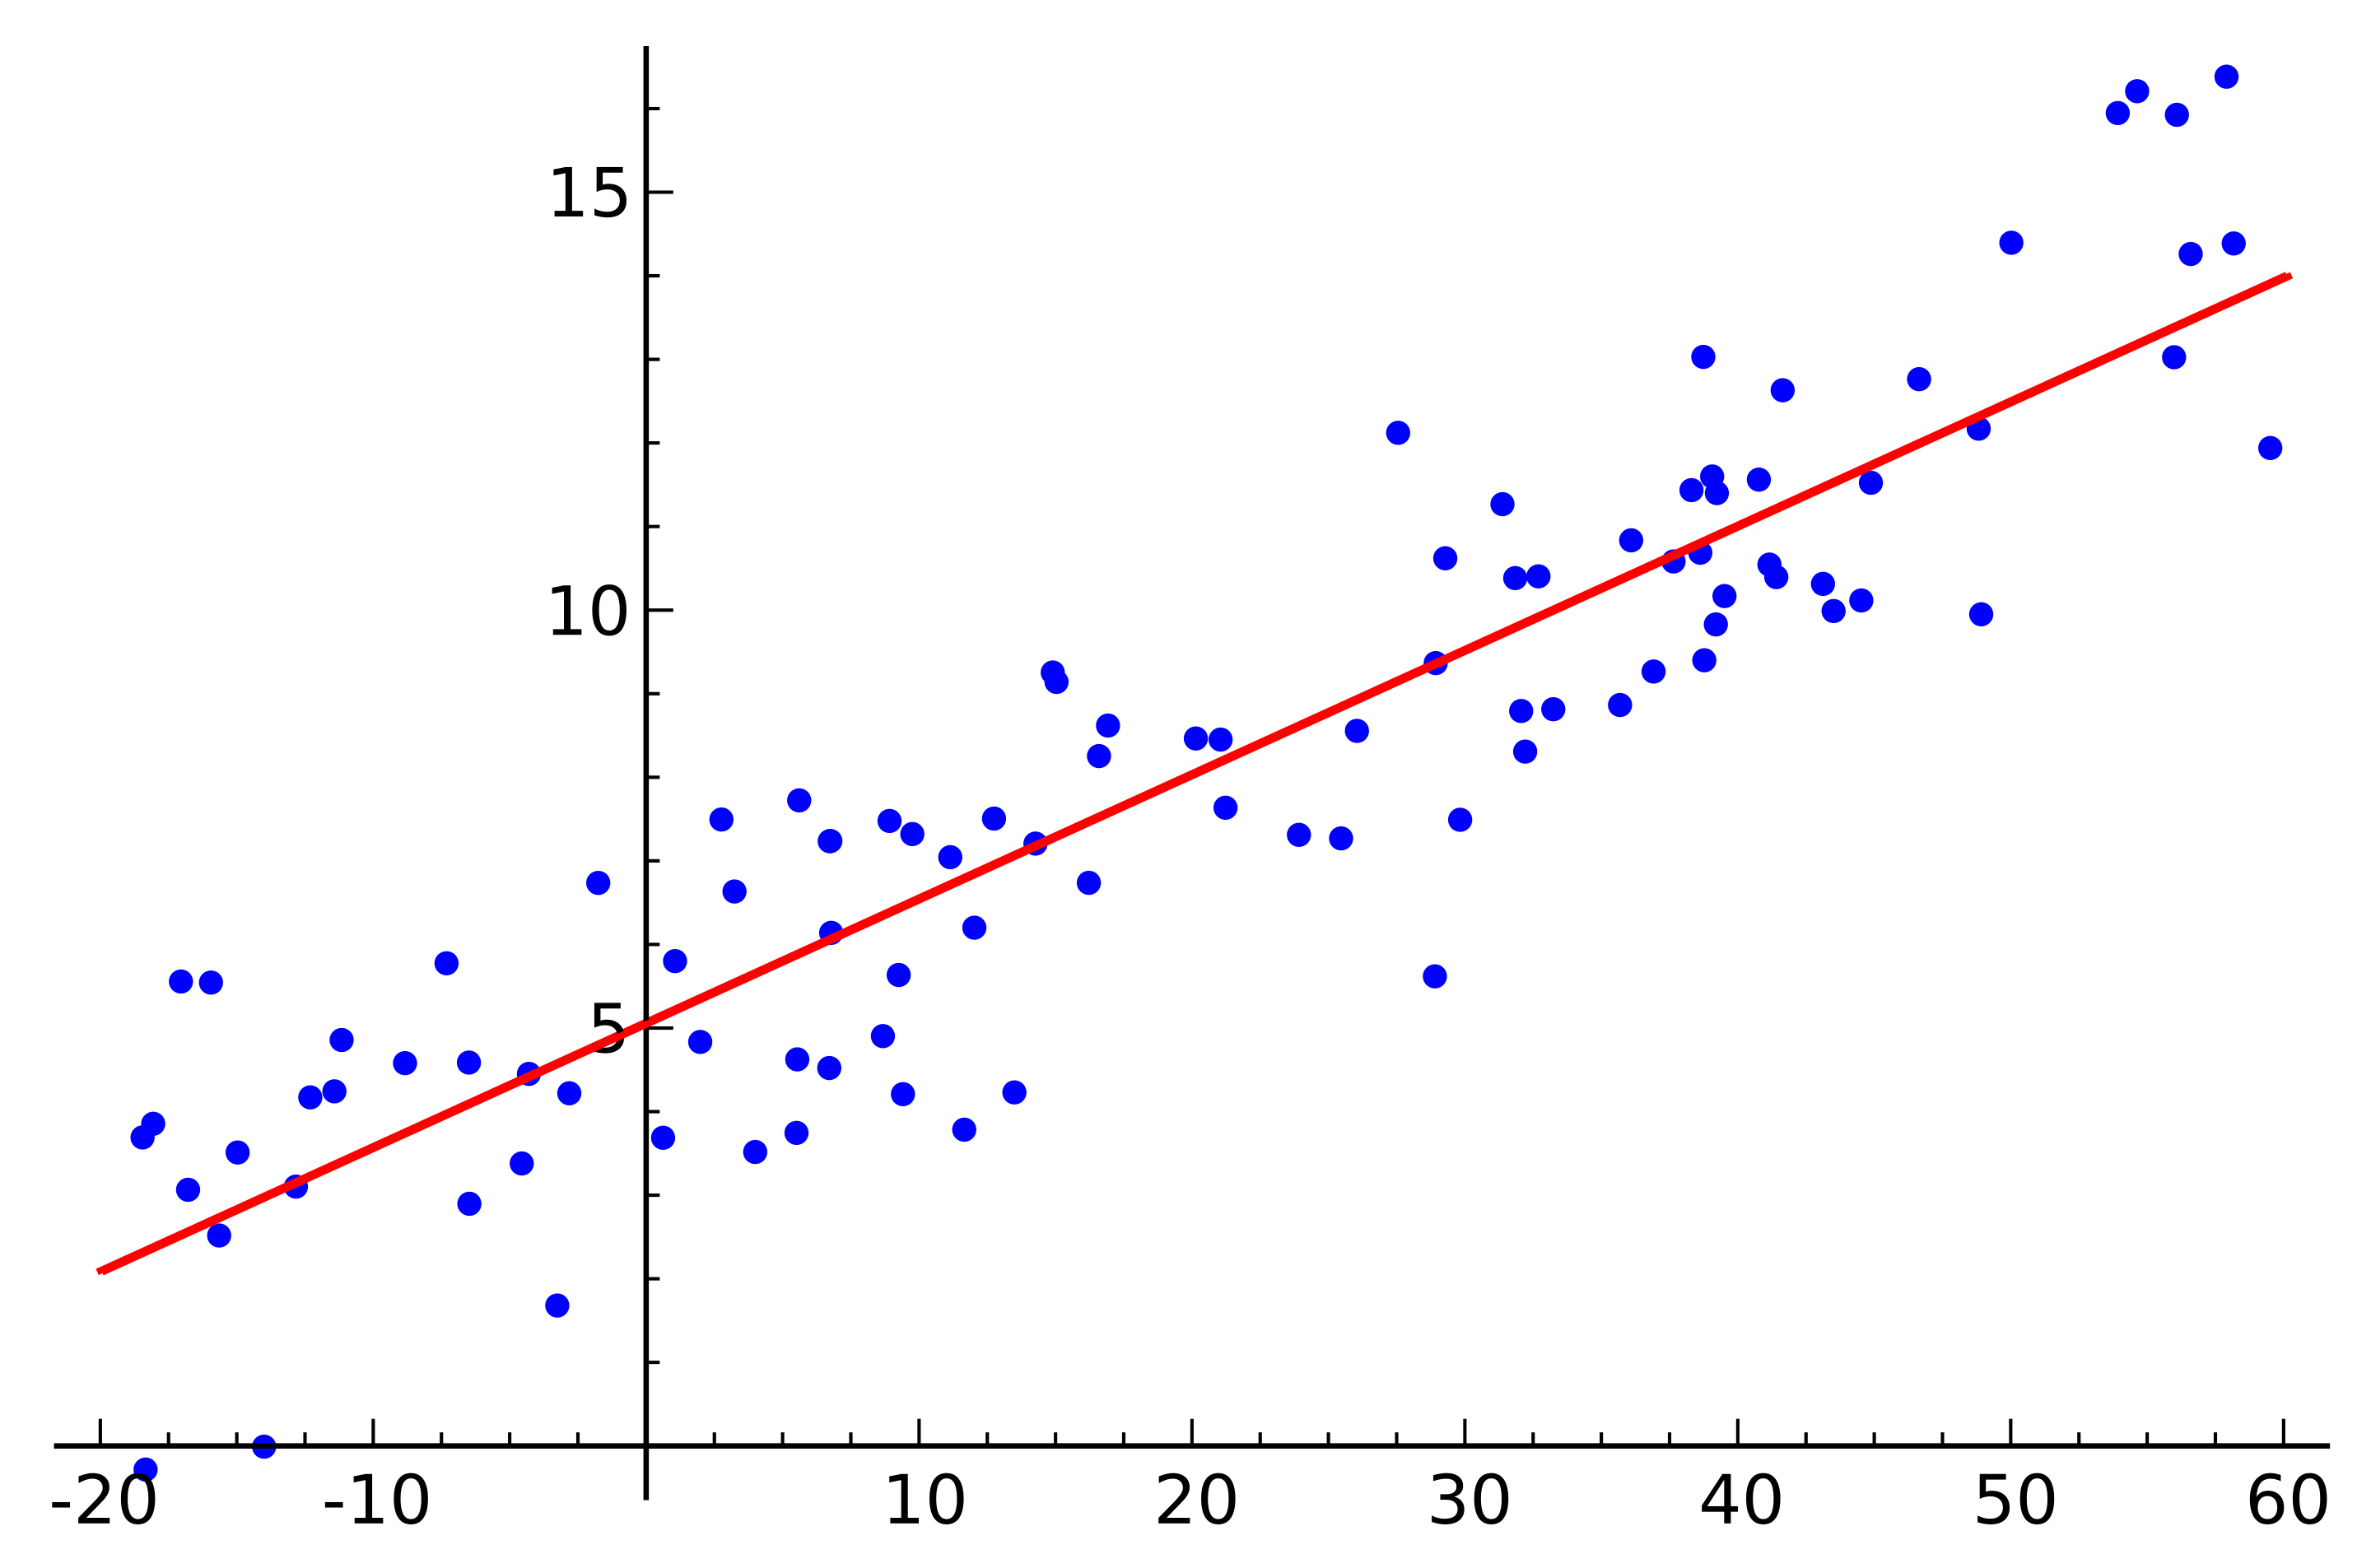
\includegraphics[scale=0.07]{2880px-Linear_regression.svg.png}
	\end{center}
\end{frame}
%-------------- end slide -------------------------------%}}}
%-------------- start slide -------------------------------%{{{ 11.5
\begin{frame}
	\centering
	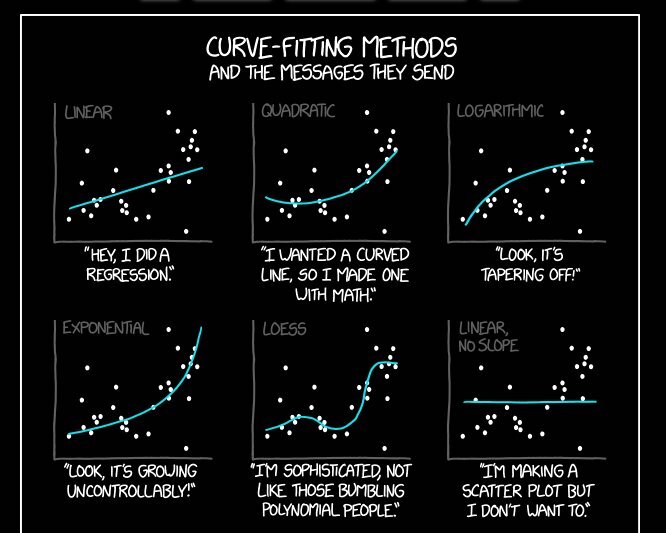
\includegraphics[scale=0.34]{xkcd_Curve_fitting2-neg.jpg}
	\\
	\footnotesize \url{https://xkcd.com/}
	% 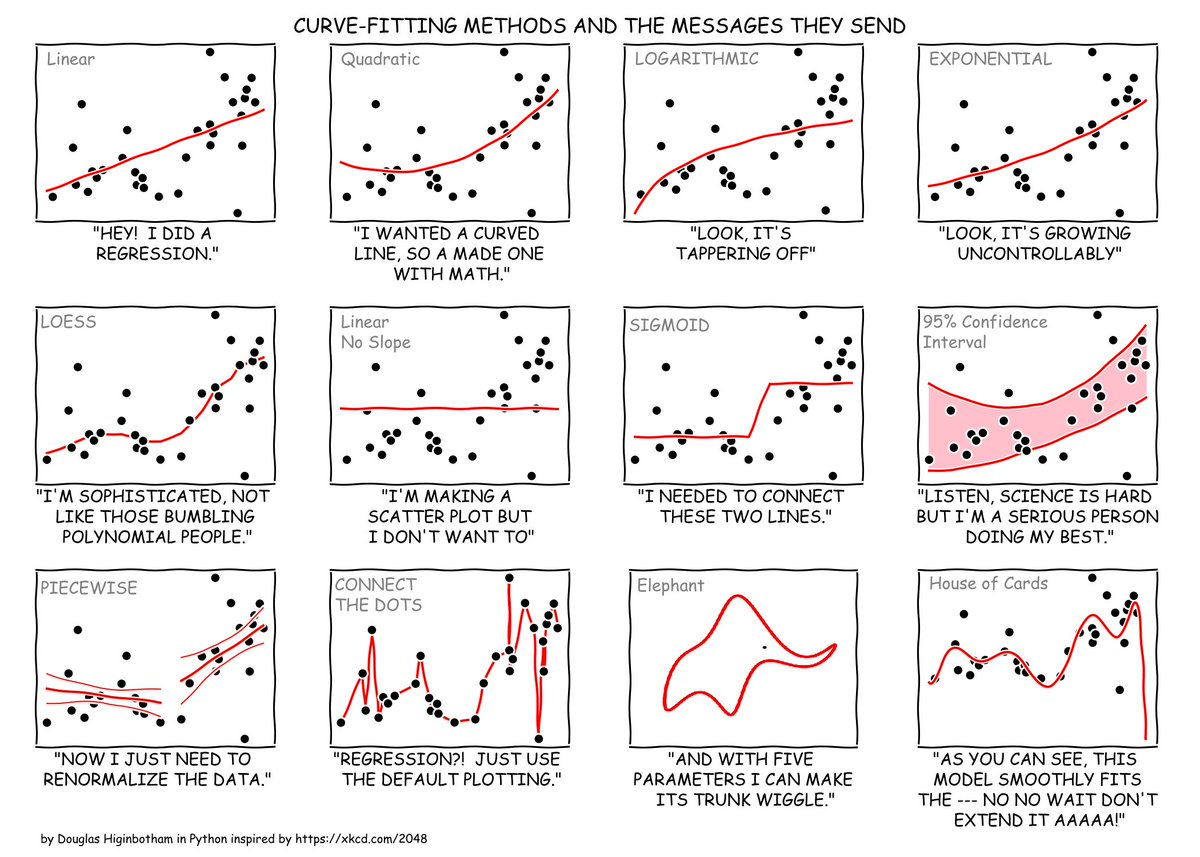
\includegraphics[scale=0.25]{xkcd_Curve_fitting.jpg}
\end{frame}
%-------------- end slide -------------------------------%}}}
%-------------- start slide -------------------------------%{{{ 11.6
\begin{frame}[fragile]{Three ways to view the same thing}

	\begin{enumerate}
		\item[]
			\[(x_1,y_1),\cdots, (x_n,y_n)\]
		\item Purely data, no probability structure assumed.
			\vfill
		\item[]
			\[(x_1,Y_1),\cdots,(x_n,Y_n)\]
		\item A random sample of size $n$, where $Y_i$ follows a distribution depending on $x_i$ which is 
			deterministic.
			\vfill
		\item[]
			\[
			(X_1,Y_1),\cdots,(X_n,Y_n)
			\]
		\item A random sample of size $n$, where $(X_i,Y_i)$ follow some joint distribution.
	\end{enumerate}
\end{frame}
%-------------- end slide -------------------------------%}}}
